\documentclass[tikz,onecolumn]{IEEEtran}



\usepackage{tikz}
\usepackage{kblocks}
\usepackage{bm}
\usepackage{csquotes}
\newcommand*{\kblocks}{\relax~\textit{k}\textsc{blocks}}
\newcommand*{\Tikz}{
    Ti\textit{k}Z
}
\newcommand*{\TikzPGF}{\relax~{Ti\textit{k}Z/\textsc{pgf}}}

\begin{document}
\title{\kblocks:\TikzPGF~Macro DEMO}
\author{
\IEEEauthorblockN{
\textsc{Oluwasegun~Somefun}~(\textbf{oasomefun@futa.edu.ng}) \\
\footnotesize{\textsc{Department of Computer Engineering, Federal University of Technology, Akure, Nigeria}}
}
}

\markboth{\kblocks~Demo. Version~01. 13, October~2019};
%%{Shell \MakeLowercase{\textit{et al.}}: Bare Demo of IEEEtran.cls for IEEE Journals}


\maketitle

\section{Introduction}
Welcome to the demo documentation of\kblocks. Desiring to typeset control block diagrams in \LaTeX~and dissatisfied with the other \LaTeX~macro packages that
can be found online, I thought: \textit{why not write my own macro package for this purpose}.

I wish to start with the question, \enquote{What is\kblocks?} The\kblocks~macro package is the product of using\TikzPGF~to
directly typeset beautiful control block diagrams and signal flow graphs in my Masters' dissertation and papers directly with \LaTeX.
Basically, it just defines a number of commands to make drawing control block diagrams using\TikzPGF~ more structured and easier. In a sense, when you
use\kblocks~you \textit{program} or typeset graphics for control block diagrams, just as you “program” graphics in your document when you use
\LaTeX~using\TikzPGF.

The powerful options offered by\TikzPGF~often intimidates beginner users not ready to spend careful time learning about\TikzPGF. Like all
\LaTeX~packages,\TikzPGF~inherits the steep learning curve of \LaTeX, that is, no \textit{what you see is what you get}.
The\kblocks~macro reduces the length of this learning curve, by focusing the graphics theme on control block diagrams only.
Fortunately this documentation as it grows and gets to be improved, will come with a number of slowly-paced
tutorials, which will guide you on creating control block diagrams with\kblocks~without your having to read the\TikzPGF~manual.

My wish is that you find it helpful. Don't forget to share and like. Please feel free to e-mail me for any improvement or suggestion with respect to
using\kblocks~and making it
useful for researchers and students in the applications and field of control theory.

\centering

\section{}
\begin{tikzpicture}
\begin{scope}
  \kStartNode[$r$]{R1}
  \kPlusMinusDown{R1}{S1}{0cm}
  \kTFRight[0cm]{S1}{B1}{$\frac{1}{s}$}
  \kMarkNodeRight[0cm]{}{B1}{N1}
  \kOutRight{N1}{Y1}{$y$}{0cm}

  \kLinkVHHVAbove[0cm]{$1$}{N1}{S1}{0}{0}
  \kLinkVHHVBelow[0cm]{$1$}{N1}{S1}{0}{0}
  \kLink[]{R1}{S1}
  \kLink[$e$]{S1}{B1}
  \kLinkn[]{B1}{N1}
\end{scope}
\end{tikzpicture}

\section{}
\begin{tikzpicture}
\begin{scope}
  \kStartNodec[$r$]{(0,5)}{R1}
  \kPlusMinusDown{R1}{S1}{0cm}
  \kTFRight[0.33cm]{S1}{B1}{$G\left( s \right)$}
  \kTFBelow[0cm]{B1}{B2}{$H\left( s \right)$}
  \kMarkNodeRight[0.2cm]{}{B1}{N1}
  \kOutRight{N1}{Y1}{$y$}{0}

  \kLinkVHTFHVBelow{$y$}{$\hat{y}$}{N1}{B2}{S1}{0}{0}{0}
  \kLink[]{R1}{S1}
  \kLink[$e$]{S1}{B1}
  \kLinkn[]{B1}{N1} 
  
  
  \kCoverRect[blue]{B1}{0.5cm}{1.5cm}{1.8cm}{1.5cm}
  \kCoverTextRight{1cm}{0.5cm}{TX1}{Closed-loop system}
  
\end{scope}
\end{tikzpicture}

\section{}
\begin{tikzpicture}
\begin{scope}
  \kStartNodec[]{(5,-5)}{R1}
  \kTFRight{R1}{M1}{$\bm{\hat{m}$}\\\textbf{PID}\\\textbf{model}}
  \kOutDown[]{M1}{um}{$u_m$}{0}
  \kScaleDistX[1.5]
  \kTFRight{M1}{C1}{$\bm{K\left(y_m,y\right)}$\\\textbf{PID}\\\textbf{controller}}
  \kTFBelowRight{0cm}{0.2cm}{C1}{P1}{$\bm{P\left(s\right)}$\\\textbf{process}}

  \kLink[$r$]{R1}{M1}
  \kLink[$y_m$]{M1}{C1}
  \kLinkHV[$u$]{C1}{P1}{north}{0}
  \kLinkHV[$y$]{P1}{C1}{south}{0}
\end{scope}
\end{tikzpicture}

\section{}
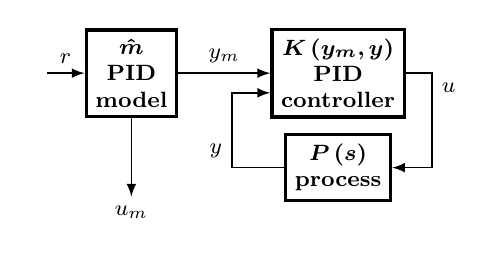
\begin{tikzpicture}
\begin{scope}
  \kStartNodec[]{(-5,-5)}{R1}
  \kTFRight{R1}{M1}{$\bm{\hat{m}$}\\\textbf{PID}\\\textbf{model}}
  \kOutDown[]{M1}{um}{$u_m$}{0}
  \kScaleDistX[1.75]
  \kTFRight{M1}{C1}{$\bm{K\left(y_m,y\right)}$\\\textbf{PID}\\\textbf{controller}}
  \kScaleDistX[1]
  \kTFBelow{C1}{P1}{$\bm{P\left(s\right)}$\\\textbf{process}}

  \kLink[$r$]{R1}{M1}
  \kLink[$y_m$]{M1}{C1}
  \kLinkHVHRight[0]{$u$}{C1}{P1}{0}{0}
  \kLinkHVHLeft[0.33]{$y$}{P1}{C1}{0}{-0.25}
\end{scope}
\end{tikzpicture}

\section{}
\begin{tikzpicture}
  \begin{scope}
    \kJumpCS{R}{$(0,0)$}

    \kJumpCSRight[-0.5cm]{R}{CR}{0}{3}
    \kJumpCSLeft[-0.5cm]{R}{CR}{0}{9}
    \kJumpCSAbove[-0.5cm]{R}{CR}{0}{12}
    \kJumpCSBelow[-0.5cm]{R}{CR}{0}{6}

    \kTFBelow{R}{C1}{\bfseries{PID}$\bm{(\cdot)}$}
    \kScaleDistX[0.67]
    \kTFBelow{C1}{P1}{$\bm{P(s)}$}
    \kScaleDistX[1]

    \kInLeft[0cm]{C1}{RI}{$r$}{0.1}

    \kMarkNodeLeft[0cm]{}{P1}{ON}
    \kLinkn[]{P1}{ON}
    \kOutLeft[-0.5cm]{ON}{Y}{$y$}{0}
    \kLinkVH[$y$]{ON}{C1}{west}{-0.1}

    \kLinkHVHRight[0]{$u$}{C1}{P1}{0}{0}

  \end{scope}
\end{tikzpicture}

\section{}
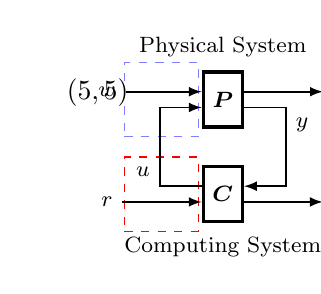
\begin{tikzpicture}
  \kJumpCS{R1}{$(5,5)$}

  \kTFRight{R1}{P1}{$\bm{P}$}
  \kScaleDistX[0.67]
  \kTFBelow{P1}{C1}{$\bm{C}$}
  \kScaleDistX[1]

  \kInLeft[]{P1}{RI}{$w$}{0.1}
  \kInLeft[]{C1}{RC}{$r$}{-0.1}

  \kLinkHVHRight[0.2]{$y$}{P1}{C1}{-0.1}{0.1}
  \kLinkHVHLeft[0.2]{$u$}{C1}{P1}{0.1}{-0.1}

  \kOutRight[0cm]{P1}{Z}{$z$}{0.1}
  \kOutRight[]{C1}{V}{$v$}{-0.1}
  
  \kCoverRect[blue!50!]{P1}{0.1cm}{0.1cm}{0.2cm}{0.2cm}
  \kCoverTextAbove{0}{0}{TX1}{Physical System}

  \kCoverRect[red]{C1}{0.1cm}{0.1cm}{0.2cm}{0.2cm}
  \kCoverTextBelow{0cm}{0cm}{TX2}{Computing System}

\end{tikzpicture}

\section{}
\begin{tikzpicture}
\kJumpCS{io}{$(0,0)$}
\kJumpCSLeft[-0.5cm]{io}{jl}{0}{9}
\kCoverRect[blue]{jl}{2cm}{2cm}{2cm}{2cm}

\end{tikzpicture}


\end{document}
